%!TEX root=../supplement.tex

\section{Canadian weather} % (fold)
\label{sec:canadian_weather}


\textcolor{blue}{We apply the different methods to the Canadian weather dataset. This Canadian weather dataset, available in the R package \texttt{fda} \cite{ramsayFdaFunctionalData2023}, provides daily temperature (°C) and precipitation (mm, rounded to $0.1$mm) recordings for $35$ Canadian cities. Originally presented in \cite{ramsayFunctionalDataAnalysis2005}, the dataset spans all days of the year, averaging data from $1960$ to $1994$. This is an example of multivariate functional data with two variables ($P = 2$), incorporating measurement errors. Figure~\ref{fig:canadian_weather} presents the data, showcasing temperature and precipitation trends across different cities.}
\begin{figure}
    \centering
    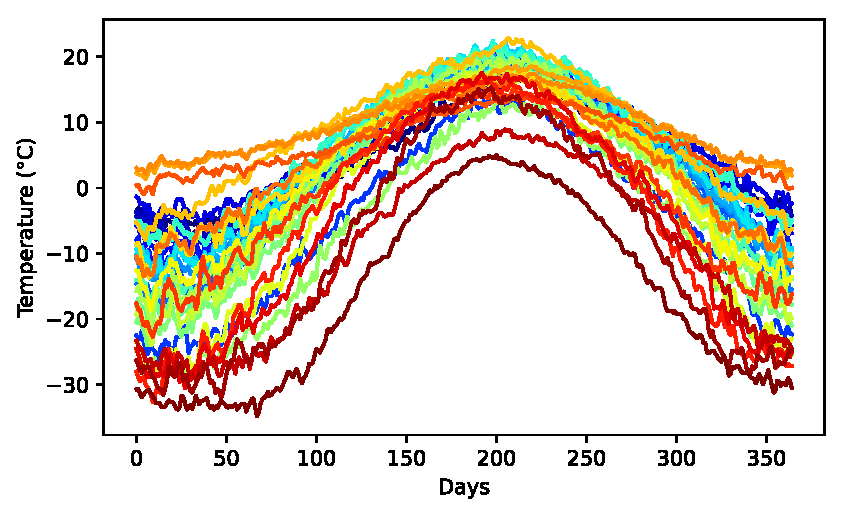
\includegraphics[width=0.49\textwidth]{figures/temperature.eps}
    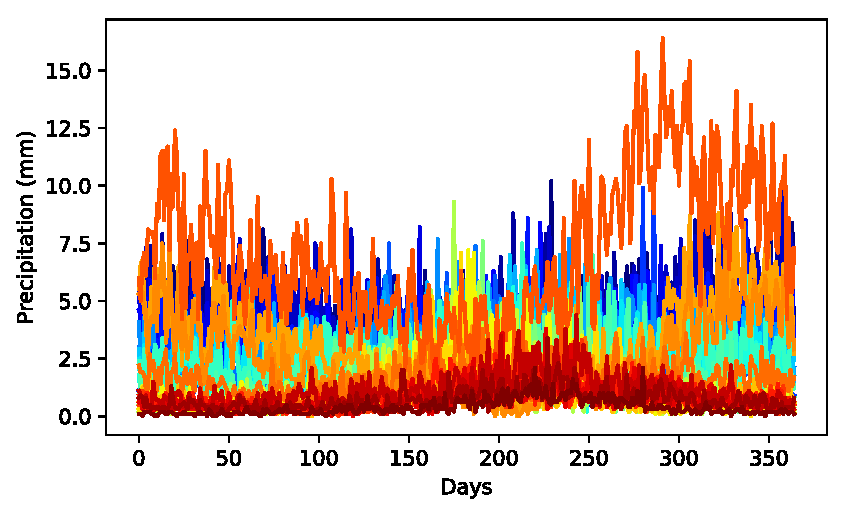
\includegraphics[width=0.49\textwidth]{figures/precipitation.eps}
    \caption{Canadian weather dataset.}
    \label{fig:canadian_weather}
\end{figure}

\textcolor{blue}{We estimate the functional principal components using the \texttt{Gram}, \texttt{(Tensor) PCA} and \texttt{2D/1D B-Splines} methods from the Canadian weather dataset. Prior to applying each method, the data was smoothed using P-splines with a fixed penalty. For the \texttt{(Tensor) PCA} method, the estimation of the multivariate eigenfunctions is based on the univariate estimation of $5$ univariate eigenfunctions. For the \texttt{2D/1D B-splines} method, the two components are expanded in $13$ B-splines.  Figure~\ref{fig:canadian_weather_eigenfunctions} presents the results of MFPCA retaining the top three principal components. Recalling that eigenfunctions are defined up to a sign, the results across all three methods are similar. Our analysis focuses on the Gram method's results. The first principal component (red) exhibits positive values for both temperature and precipitation, indicating that weather stations with positive scores will experience above-average temperatures and precipitation. This effect is more pronounced during winter than summer, as the eigenfunctions approach zero during the summer months. Similar interpretations can be applied to the remaining eigenfunctions.}
\begin{figure}
    \centering
    \begin{subfigure}[b]{0.3\textwidth}
    \centering
    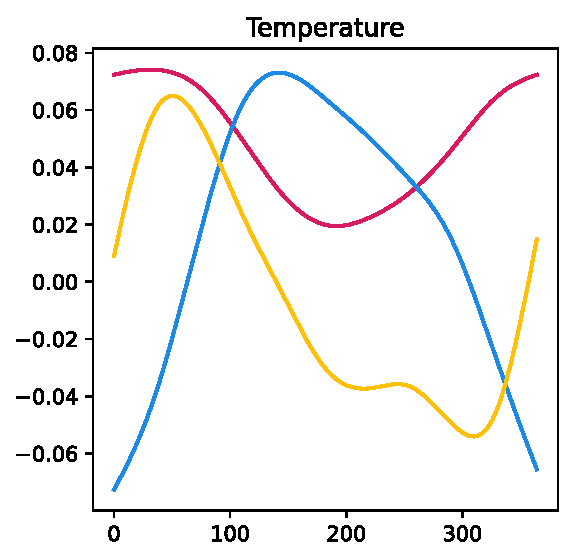
\includegraphics[width=\textwidth]{figures/eigen_temp_gram.eps}
    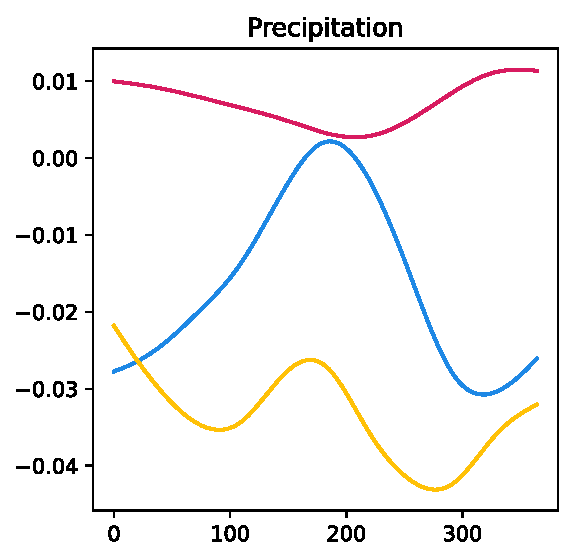
\includegraphics[width=\textwidth]{figures/eigen_prec_gram.eps}
    \caption{\texttt{Gram} method.}
    \end{subfigure}
    \hfill
    \begin{subfigure}[b]{0.3\textwidth}
    \centering
    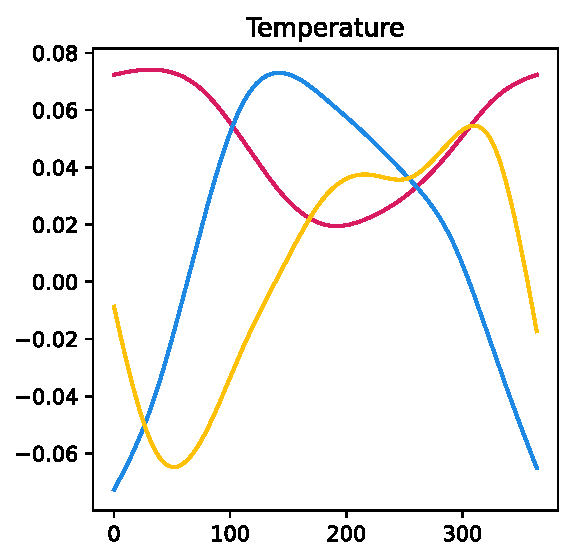
\includegraphics[width=\textwidth]{figures/eigen_temp_cov.eps}
    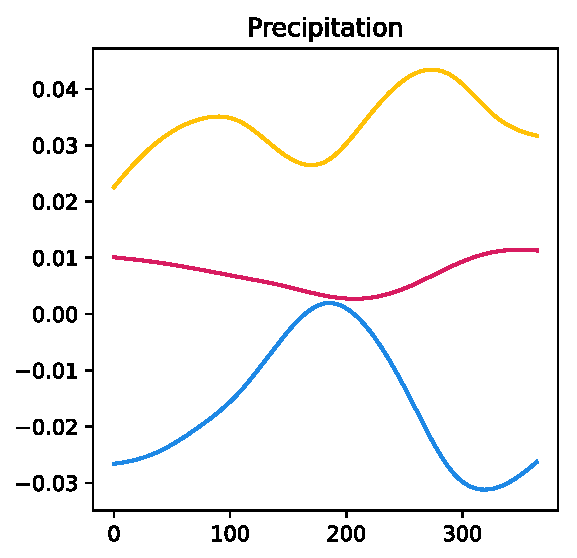
\includegraphics[width=\textwidth]{figures/eigen_prec_cov.eps}
    \caption{\texttt{(Tensor) PCA} method.}
    \end{subfigure}
    \hfill
    \begin{subfigure}[b]{0.3\textwidth}
    \centering
    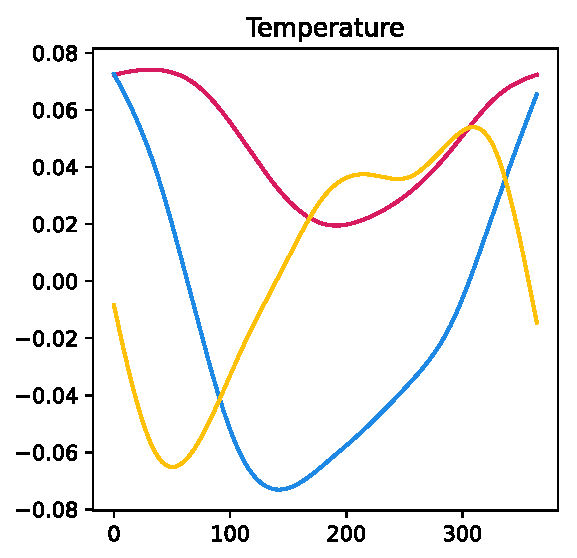
\includegraphics[width=\textwidth]{figures/eigen_temp_psplines.eps}
    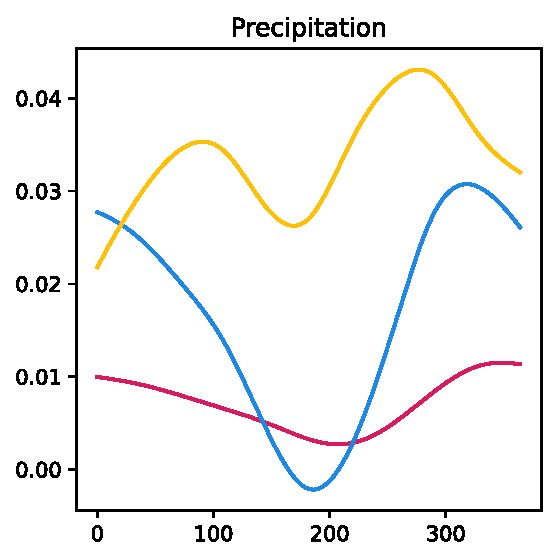
\includegraphics[width=\textwidth]{figures/eigen_prec_psplines.eps}
    \caption{\texttt{2D/1D B-Splines} method.}
    \end{subfigure}
    \caption{The estimated eigenfunctions for the Canadian weather dataset using the different methods.}
    \label{fig:canadian_weather_eigenfunctions}
\end{figure}


% section canadian_weather (end)